La résolution du problème via Matlab nous montre que, lorsque le nombre d'ouvriers est constant, l'usine tourne à plein régime en permanence, accumule beaucoup de stock et de retard, jusqu'à parfois devoir recourir à la sous-traitance pour livrer dans les temps.

Il semble évident qu'un important bottleneck se situe au niveau du nombre d'ouviers disponibles, d'où l'ajout, à partir de la question 7, du nombre variable d'ouviers.

On notera que la fonction coût diffère d'une constante entre le rapport le programme Matlab; en effet, dans ce dernier, la fonction tient compte du coût horaire du travail de tous les employés sur les différentes semaines. Ce simple ajout permet d'avoir le coût réel de la production.

\begin{figure}[h]
    \centering
    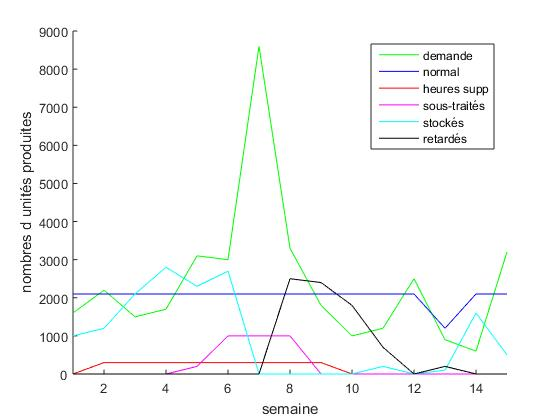
\includegraphics[width=0.8\textwidth]{graphes/graphq3.jpg}
    \caption{Graphe de la production à personnel constant}
    \label{fig:q3}
\end{figure}
